\subsection{Diferenças sobre linguagens convencionais}
\label{diferencasdsl}

Segundo \citeonline{dslengineering}, o propósito das \gls{DSL} é de atender a um domínio específico, são construídas para resolver uma classe específica de problemas. De outro lado as \gls{GPL} são voltadas aos desenvolvedores para resolver qualquer tipo de problema computável:

\begin{citacao}
As Linguagens de Programação de Uso Geral (GPLs) são um meio para programadores instruírem computadores.Todas podem ser usadas para implementar qualquer coisa computável com uma máquina de Turing. Isso também significa que qualquer coisa expressável com uma linguagem de programação completa de Turing também pode ser expressa em qualquer outra linguagem de programação completa de Turing. Nesse sentido, todas as linguagens de programação são intercambiáveis. \cite{dslengineering}
\end{citacao}

Para \citeonline{ghosh2011dsl}, projetar uma DSL não é uma tarefa tão assustadora quanto projetar uma linguagem de programação de uso geral. Pois tem foco limitado e é restrita apenas ao domínio que está sendo modelado.

Enquanto \gls{GPL} são flexíveis, as \gls{DSL} sacrificam a flexibilidade em benefício da produtividade e da concisão de programas relevantes em um domínio específico. As \gls{GPL}s são utilizadas em domínios maiores e complexos, do outro lado são trabalhado problemas menores e bem definidos \cite{dslengineering}. Algumas dessas diferenças podem ser observadas na  Figura \ref{fig:gplvsdsl}.

\begin{figure}[h!]
\centering

\caption{\textmd{DSL vs GPL}}
\label{fig:gplvsdsl}
\fcolorbox{gray}{white}{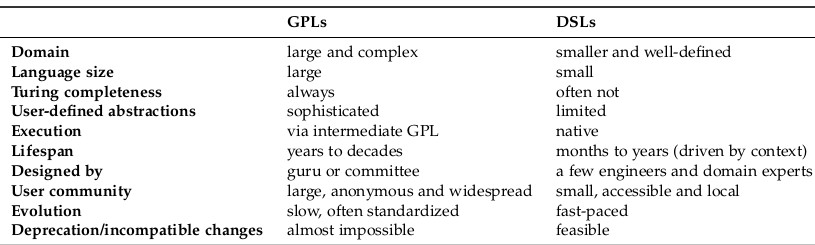
\includegraphics[width=\textwidth]{chapters/fundamentacao/imagens/gplvsdsl.jpg}}

\par\medskip\textbf{Fonte:} \citeonline{dslengineering}. \par\medskip
\end{figure}


Existem situações em que usuários precisam inserir algumas regras  %citar novak



\subsection{Vantagens e desvantagens de uso de DSL}
\label{beneficiosdsl}


\subsection{Ferramentas de construção de DSL}
\label{ferramentasdsl}